\subsection{run\_AGC - WIP}
This example was designed to explore how two area's AGC routine would respond to a load step.
At $t=2$, a 0.5 PU real load step occurs on Bus 4 in Area 1.
AGC action was scheduled to begin at $t=25$ and then again every 15 seconds there after.

\subsubsection{run\_AGC Result Summary - WIP}
The 120 second simulation is shown to capture transients due to the load step, governor action arresting frquency change, and then AGC acting to restore system frequency and interchange values.


\begin{figure}[H]
	\centering
	\footnotesize
	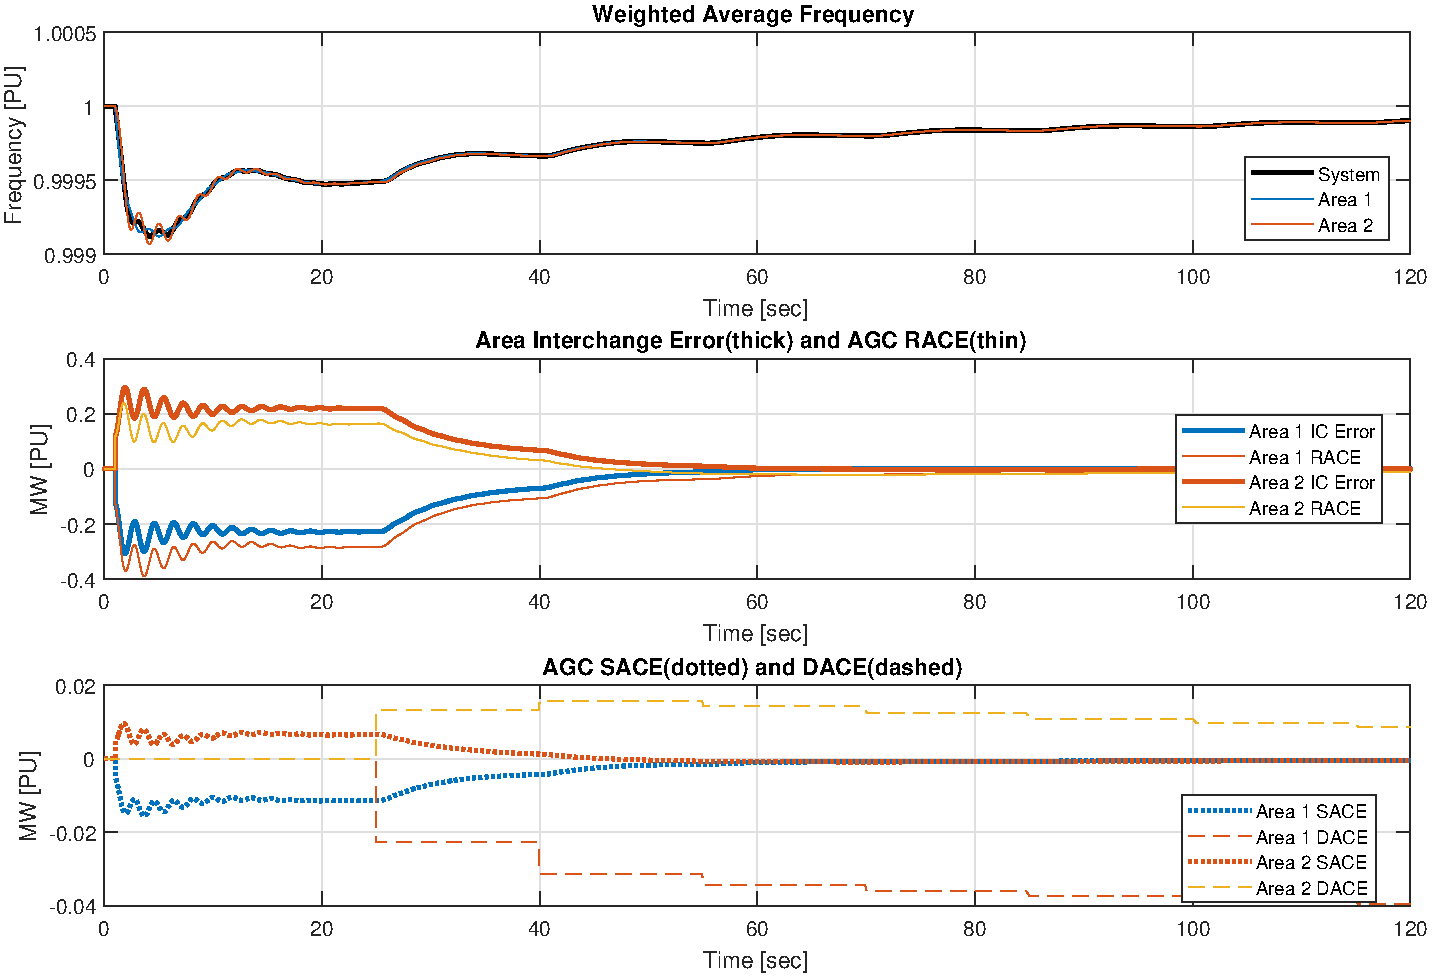
\includegraphics[width=\linewidth]{examples/agc/run-AGC-1}
	\caption{Final live Plot output from run\_AGC.}
	\label{fig: runAGC liveplot}
\end{figure}%\vspace{-1 em}

\begin{figure}[H]
	\centering
	\footnotesize
	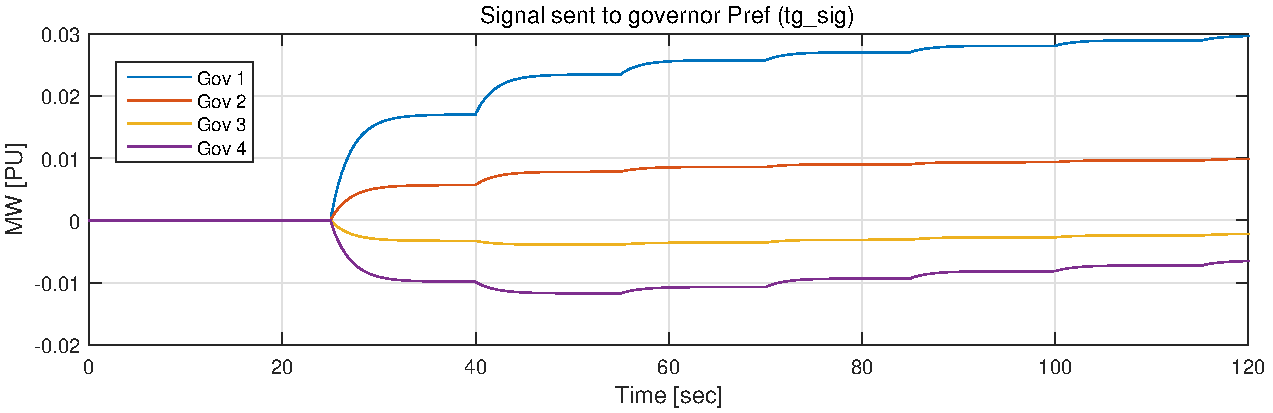
\includegraphics[width=\linewidth]{examples/agc/run-AGC-2}
	\caption{Governor modulation signals sent in run\_AGC.}
	\label{fig: runAGC tg}
\end{figure}%\vspace{-1 em}

\begin{figure}[H]
	\centering
	\footnotesize
	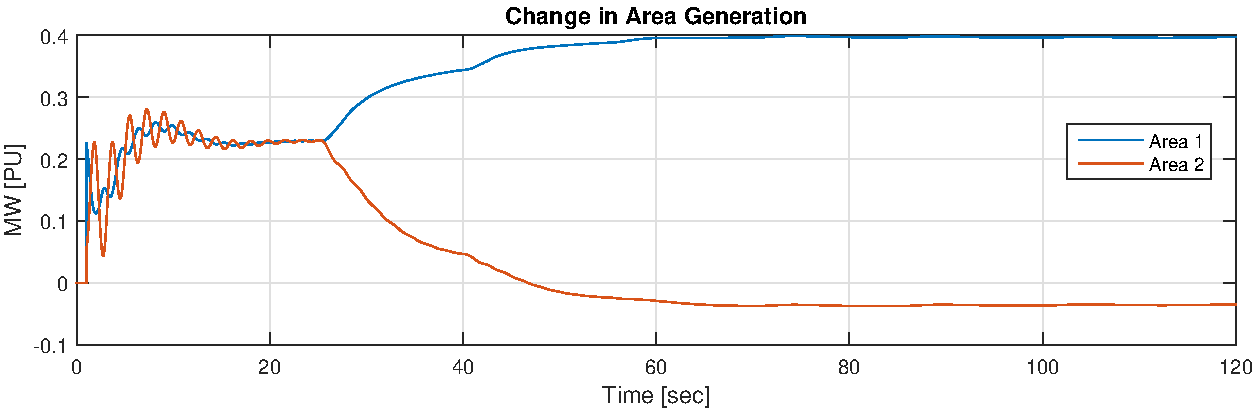
\includegraphics[width=\linewidth]{examples/agc/run-AGC-3}
	\caption{Change in area generation during run\_AGC.}
	\label{fig: runAGC area gen}
\end{figure}%\vspace{-1 em}


\begin{figure}[H]
	\centering
	\footnotesize
	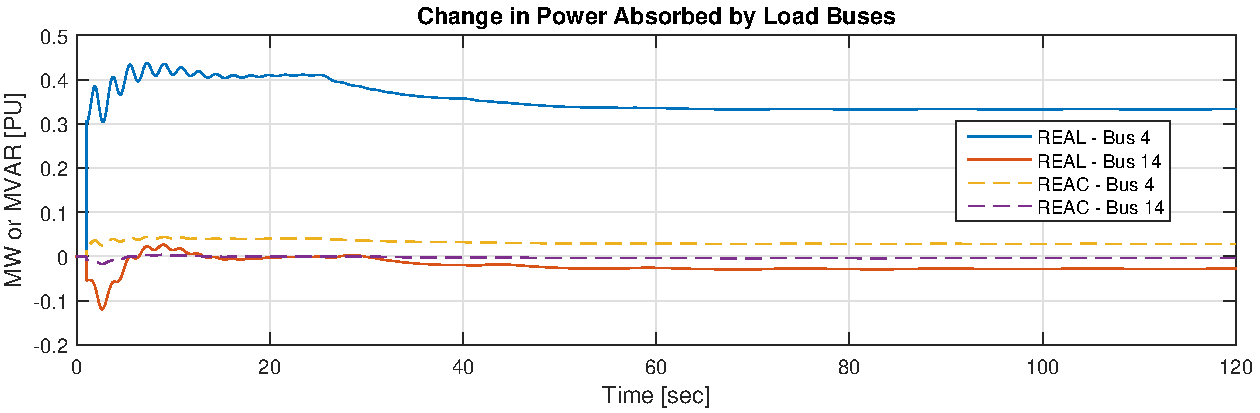
\includegraphics[width=\linewidth]{examples/agc/run-AGC-4}
	\caption{Power absorbed by loads during run\_AGC.}
	\label{fig: runAGC power}
\end{figure}%\vspace{-1 em}

\begin{figure}[H]
	\centering
	\footnotesize
	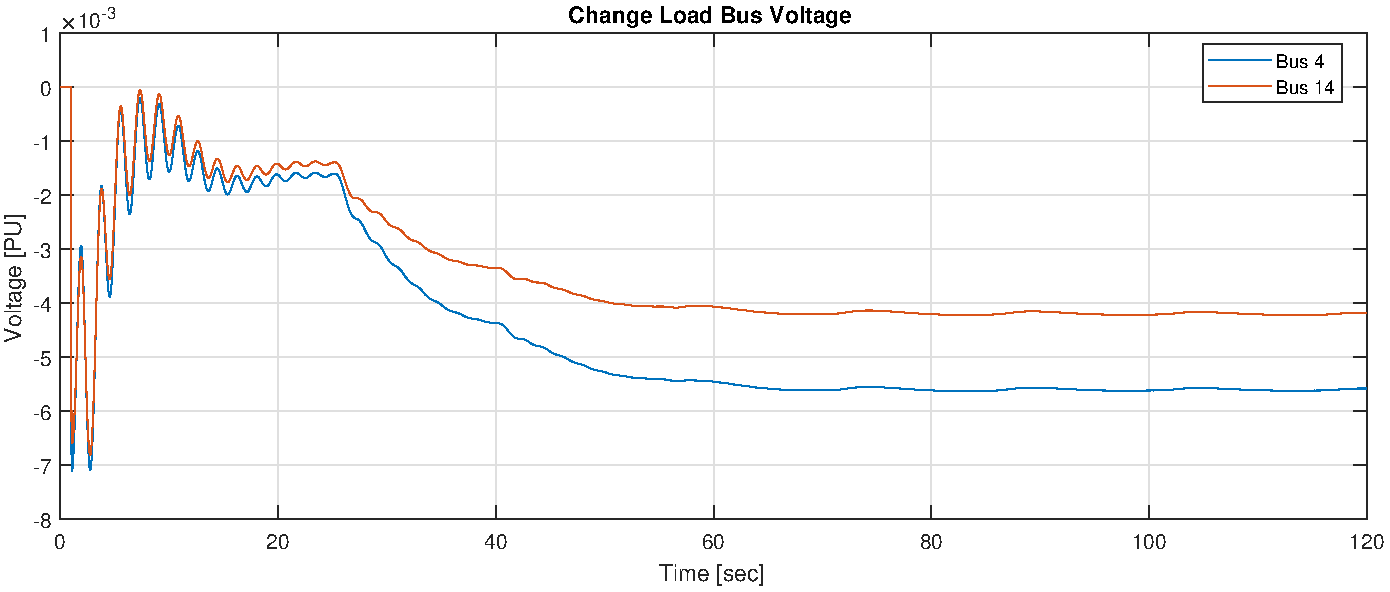
\includegraphics[width=\linewidth]{examples/agc/run-AGC-5}
	\caption{Load bus voltage change during run\_AGC.}
	\label{fig: runAGC bus v}
\end{figure}%\vspace{-1 em}